\documentclass[compress, usepdftitle=false]{beamer}
\usepackage[utf8]{inputenc}
\usepackage[T1]{fontenc}
\usepackage{lmodern}
\usepackage[french]{babel}
\usepackage{amsfonts}
\usepackage{amsmath}
\usepackage{amsthm}

\useinnertheme{default}
\useoutertheme{miniframes}
\usecolortheme{beaver}
\usefonttheme[onlymath]{serif}
\setbeamercovered{transparent}
\setbeamertemplate{section in toc}[sections numbered]

\newcommand{\cont}{\mathcal{C}^0}
\newcommand{\cun}{\mathcal{C}^1}
\newcommand{\cinf}{\mathcal{C}^\infty}
\newcommand{\R}{\mathbb{R}}
\newcommand{\N}{\mathbb{N}}

\newtheorem{thm}{Théorème}
\newtheorem{cor}{Corollaire}
\newtheorem{lemm}{Lemme}
\theoremstyle{definition}
\newtheorem{defn}{Définition}

\author{Farid Arthaud}
\title{Théorie des Catastrophes}
\date{}
\institute{TIPE 2018}

\begin{document}
\section*{Introduction}

\frame{\titlepage}

\frame{\tableofcontents}

\begin{frame}{Contexte historique}
    \begin{itemize}
        \item Hassler \textsc{Whitney}: classification pour les dimensions inférieures à deux (1955)
        \item René \textsc{Thom}: \textit{Stabilité structurelle et morphogenèse} (1972)
        \item Cristopher \textsc{Zeeman}: Recherche intensive aux cotés de \textsc{Thom}
        \item Popularisation (années 70) et applications diverses (biologie, sociologie, ...)
        \item Controverse, remise en question de la pertinence des applications
    \end{itemize}
    \begin{quote}<2>
        ``Les choses qui changent soudainement, par à-coups, ont longtemps résisté à toute analyse mathématique.
        Une méthode dérivée de la topologie décrit ces phénomènes comme des exemples de sept `catastrophes élémentaires'.'' - C. \textsc{Zeeman}
    \end{quote}
\end{frame}

\begin{frame}{Exemple: le baigneur}
    \begin{columns}[T]
        \begin{column}{5cm}
            \begin{itemize}[<+->]
                \item Contrôle absolu sur la précision
                \item `Virage' soudain et incontournable lors du réglage du paramètre
            \end{itemize}

            \pause[3]
            \alert{Explication}: Disparition d'un équilibre d'un système physique

            \pause
            \alert{Objectif}: Saisir la classification des catastrophes établie par \textsc{Thom} en faibles dimensions et quelques applications
        \end{column}
        \begin{column}{5cm}
            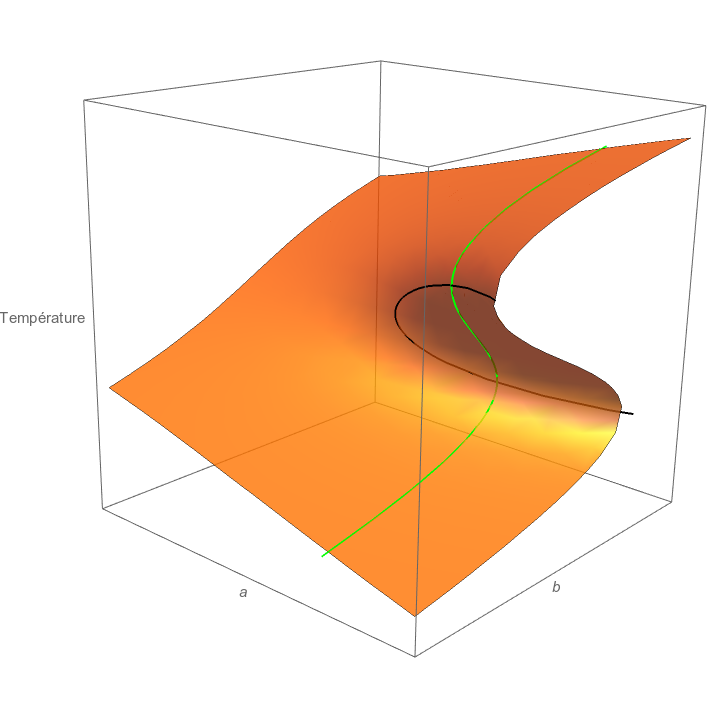
\includegraphics[width=1.05\linewidth,height=1.05\textheight,keepaspectratio]{images/cusp_temp.png}
        \end{column}
    \end{columns}
\end{frame}

\section[Exemples]{Premiers exemples}

\subsection{La machine de \textsc{Zeeman}}
\begin{frame}{Expérience}
    \includegraphics<1>[width=\linewidth,height=\textheight,keepaspectratio]{images/montage_loq.jpg}
    \includegraphics<2>[width=\linewidth,height=\textheight,keepaspectratio]{images/eq_haut_loq.jpg}
    \includegraphics<3>[width=\linewidth,height=\textheight,keepaspectratio]{images/eq_bas_loq.jpg}
\end{frame}

\begin{frame}{Analyse théorique}
    \begin{onlyenv}<1-3>
        \includegraphics<1-3>[width=\linewidth,height=0.8\textheight,keepaspectratio]{images/zeeman_sketch.jpg}

        Un calcule donne une \alert{énergie potentielle} de la forme:

        $$E_p(a, b, \theta)  = \Lambda \times (\frac{1}{4}\theta^4+\frac{a}{2}\theta^2+b\theta) + E_{p,0} + g(\theta)$$
        où $g(0)=g'(0)=g''(0)=g^{(3)}(0)=g^{(4)}(0)=0$.

        \pause
        \alert{Positions d'équilibre} ou points critiques:

        $$\theta^3+a\theta+b=0$$

        \pause
        \textit{Remarque}: $1$ ou $3$ positions d'équilibre pour chaque couple $(a,b)$
    \end{onlyenv}

    \begin{figure}\includegraphics<4>[width=\linewidth,height=0.8\textheight,keepaspectratio]{images/cusp_zeeman.png}
    \includegraphics<5>[width=\linewidth,height=0.8\textheight,keepaspectratio]{images/cusp_zeeman_top.png}\end{figure}
\end{frame}

\subsection{Surfaces en trois dimensions}
\begin{frame}{Projection sur le plan}
    On considère $f:\R^3\to\R, \cinf$ et la surface $V = \{ (x,y,z)\mid f(x,y,z)=0 \} \subseteq \R^3$

    \pause
    Projection de cette surface sur le plan $\{(x,y)\} = \R^2$

    Le \alert{contour apparent} est l'ensemble des points $x$ tels que $\frac{\partial f}{\partial z}(x) = 0$
\end{frame}

\begin{frame}{Points-pli et points-fronce}
    \begin{columns}[T]
        \begin{column}{5cm}
            \alert{Point-pli}

            $a$ est point-pli s'il existe des coordonnées dans lesquelles
            $$\pm f(x, y, z) = z^2 - y$$

            \uncover<3-4>{
                \alert{Point-fronce}

                $a$ est point-fronce s'il existe des coordonnées dans lesquelles
                $$f(x,y,z) = z^3 - xz - y$$}
        \end{column}
        \begin{column}{5cm}
            \includegraphics<1>[width=5cm,keepaspectratio]{images/fold_front.png}
            \includegraphics<2>[width=5cm,keepaspectratio]{images/fold_top.png}
            \includegraphics<3>[width=5cm,keepaspectratio]{images/cusp_front.png}
            \includegraphics<4>[width=5cm,keepaspectratio]{images/cusp_side.png}
        \end{column}
    \end{columns}
\end{frame}

\begin{frame}{Contour d'une surface}
    \begin{thm}
        Si $f$ est choisie ``au hasard'', alors:
        \begin{enumerate}[<+->]
            \item $\{f=0\}$ est une sous-variété de dimension deux (\alert{surface})
            \item Son contour apparent $\{f=0\}\cap \left\{\frac{\partial f}{\partial z}=0\right\}$ est une sous-variété de dimension un (\alert{courbe})
            \item Tous les points ``particuliers'' sont des points-plis ou points-fronces, et les points-fronces sont isolés
        \end{enumerate}
    \end{thm}
\end{frame}

\section{Catastrophes}

\subsection{Variétés et points critiques}
\begin{frame}{Points critiques}
    \begin{onlyenv}<1-3>
        Soit $f: E \to F, \cun$
        \begin{defn}
            Un point critique pour $f$ est un point $a$ où $df_a$ n'est \alert{pas surjective}.
        \end{defn}

        \pause
        \alert{Exemples:}
        \begin{description}[<+->]
            \item[$\R\to\R$:] $a$ point critique $\iff f'(a) = 0$
            \item[$\R^n\to\R$:] $a$ point critique $\iff \forall k, \frac{\partial f}{\partial x_k}(a) = 0$
        \end{description}
    \end{onlyenv}

    \only<4-5>{\alt<4>{$$f:x\mapsto x^2$$}{$$f:(x,y)\mapsto x^2+y^2$$}}

    \begin{figure}\includegraphics<4>[width=5cm,keepaspectratio]{images/x_deux.png}
    \includegraphics<5>[width=5cm,keepaspectratio]{images/x_deux_y_deux.png}\end{figure}
\end{frame}

\begin{frame}{Sous-variétés}
    \begin{defn}
        Une \textbf{sous-variété} $V$ de $\R^n$ est un ensemble qui est localement descriptible par un \alert{système non dégénéré d'équations locales}, soit $m$ équations indépendantes.
        \begin{enumerate}[<+->]
            \item pour un voisinage de $a$, $x\in V \iff \Phi_1(x)=...=\Phi_m(x)=0$
            \item $d\Phi_{1,a},...,d\Phi_{m,a}$ forment un système libre de formes linéaires.
        \end{enumerate}

        \pause[3]
        $m$ est la \textbf{codimension} de la sous-variété, supposée être la même en tout point de $V$ par la suite
    \end{defn}

    \pause
    \begin{thm}
        Une sous-variété de dimension $p$ admet en tout point un \alert{espace tangent} de dimension $p$.

        C'est l'intersection \alert{transverse} des $ker(d\phi_{1,a}),...,ker(d\phi_{m,a})$.
    \end{thm}
\end{frame}

\subsection{Transversalité et généricité}
\begin{frame}{Intersections transverses}
    \begin{onlyenv}<1-2,6>
        \uncover<1-2>{
            \begin{defn}
                Deux sous-espaces $F$ et $G$ sont dits d'\textbf{intersection transverse} si $F+G=E$.
            \end{defn}

            \pause
            \alert{Caractérisation}: Toutes translations des espaces s'intersectent}

        \uncover<6>{Pour des \textbf{variétés et des fonctions}, transversalité si les \alert{espaces tangents} sont transverses en tout point de l'intersection}
    \end{onlyenv}

    \includegraphics<3>[width=\linewidth,height=0.8\textheight,keepaspectratio]{images/2DTransverse.png}
    \includegraphics<4>[width=\linewidth,height=0.8\textheight,keepaspectratio]{images/3D_trans.png}
    \includegraphics<5>[width=\linewidth,height=0.8\textheight,keepaspectratio]{images/3D_non_trans.png}
\end{frame}

\begin{frame}{Généricité, Théorèmes de transversalité}
    \begin{onlyenv}<1-3,6>
        \begin{uncoverenv}<1-3>
            Comment définir le \alert{``hasard''} sur des ensembles de fonctions?

            \pause
            \begin{defn}
                Une propriété sur un ensemble $E$ est dite \textbf{générique} si elle est vraie sur une intersection d'ouverts denses.
            \end{defn}

            $f$ choisie ``au hasard'' $\iff$ $f$ vérifie une \alert{propriété générique}

            \pause
            \begin{thm}
                Une intersection transverse de sous-variétés est une sous-variété.
            \end{thm}
        \end{uncoverenv}

        \uncover<6>{\begin{thm}[de transversalité faible]
            Si $X$ est une sous-variété de $W$, une application $V\to W$ choisie ``au hasard'' (par généricité) sera transverse à $W$.
        \end{thm}}
    \end{onlyenv}

    \begin{figure}\includegraphics<4>[width=\linewidth, height=0.8\textheight, keepaspectratio]{images/var_trans.png}
    \includegraphics<5>[width=\linewidth, height=0.8\textheight, keepaspectratio]{images/var_non_trans.png}
    \includegraphics<7>[width=\linewidth, height=0.8\textheight, keepaspectratio]{images/trans_fun.png}\end{figure}
\end{frame}

\section[Classification]{Théorème de classification}

\subsection{Théorème de transversalité de \textsc{Thom}}
\begin{frame}{Espace des germes}
    \begin{onlyenv}<1-2>
        \begin{defn}
            Un \textbf{$k$-jet} de $f$ en $x$ correspond aux premiers termes du développement de Taylor d'une fonction:
            $$j^k_x f = \left(f(x), df_x,...,d^kf_x\right)$$

            L'\textbf{espace des germes} $J^r(E,F)$ correspond aux couples $(a, j^r_af)$
        \end{defn}

        \pause[2]
        Permet d'exprimer des \textit{équations différentielles} comme des sous-variétés:
        $$f'(x)=f(x) \iff (x,j^1_xf) \in \{(a,b,c) \mid b=c \} \subseteq J^1(\R,\R) \simeq \R^3$$
    \end{onlyenv}

    \only<3-4>{\alt<3>{$$\{(a,b,c) \mid b=c \} \subseteq J^1(\R,\R) \simeq \R^3$$}{$$j^1_x(exp) =  (x, e^x, e^x) \in \{(a,b,c) \mid b=c \}$$}}

    \begin{figure}\includegraphics<3>[width=\linewidth, height=0.6\textheight, keepaspectratio]{images/equadiff.png}
    \includegraphics<4>[width=\linewidth, height=0.6\textheight, keepaspectratio]{images/exponential.png}\end{figure}
\end{frame}

\begin{frame}{Le théorème de transversalité de \textsc{Thom}}
    \begin{onlyenv}<1-4>
        \begin{thm}[de transversalité de \textsc{Thom}]
            Pour une sous-variété $W$ d'un espace des germes $J^r(E,F)$ donnée, une fonction $f$ choisie ``au hasard'' (générique) aura $j^rf$ transverse à $W$.
        \end{thm}

        \pause
        \textbf{Exemple}: $\{(a,b,c) \mid b=c \}$ est une sous-variété de dimension $2$ de $J^1(\R,\R)$ décrivant $f'=f$

        \pause
        Espace tangent en $(a,b,b)$: $\left((1,0,0), (0,1,1)\right)$

        Espace tangent de $j^1f$ en $j^1_xf$: $(1,f'(x),f''(x)) \notin \left((1,0,0), (0,1,1)\right)$

        \pause
        Une fonction $f$ choisie ``au hasard'' en chaque point soit: ne vérifie pas $f'(x)=f(x)$, soit le vérifie en un point isolé
    \end{onlyenv}

    \begin{figure}\includegraphics<5>[width=\linewidth, height=0.8\textheight, keepaspectratio]{images/equadiff.png}\end{figure}
\end{frame}

\subsection{Théorème de \textsc{Whitney}}
\begin{frame}{Retour au cas des surfaces}
    On revient au cas de $V = \{ (x,y,z)\mid f(x,y,z)=0 \} \subseteq \R^3$

    \pause
    \begin{itemize}
        \item $\{ f=0 \}$ est une sous-variété de codimension $1$ de $J^1(\R^3,\R) \simeq \R^7$
        \item $\{ f=0 \}\cap \left\{ \frac{\partial f}{\partial z}=0 \right\}$ est une sous-variété de codimension $2$
    \end{itemize}

    \pause
    \begin{cor}[\textsc{Whitney}]
        Si $f$ est choisie ``au hasard'', alors:
        \begin{enumerate}
            \item $\{f=0\}$ est une sous-variété de \textbf{codimension un} (\alert{surface})
            \item Son contour apparent $\{f=0\}\cap \left\{\frac{\partial f}{\partial z}=0\right\}$ est une sous-variété de \textbf{codimension deux} (\alert{courbe})
            \item Tous les points \textbf{critiques} sont des points-plis ou points-fronces, et les points-fronces sont isolés
        \end{enumerate}
    \end{cor}
\end{frame}

\end{document}

\subsection{Réecriture au voisinage d'un point critique}
\begin{frame}{Lemmes d'\textsc{Hadamard}, de \textsc{Morse}, inversion locale}
    \begin{thm}[inversion locale]
        Si $a$ n'est pas un point critique, il existe des coordonnées locales telles que $f(x)=f(a)+x$.
    \end{thm}
    \begin{lemm}{(de \textsc{Hadamard})}
        Il existe un voisinage de $0$ sur lequel $f$ peut s'écrire: $f(x)=x_1g_1(x)+...+x_ng_n(x)$ avec $g_i(0) = \frac{\partial f}{\partial x_i}(0)$.

        Si $df_0=0$, on peut réitérer cela et écrire (toujours sur un voisinage de $0$):

        $$f(x)=\sum_{1\leq i,j \leq n} x_ix_jh_{ij}(x)$$
    \end{lemm}
    \begin{lemm}{(de \textsc{Morse})}
        Si $f$ admet un point critique non dégénéré en $u$, alors il existe un voisinage de $u$ et des coordonnées centrées en $u$ $y=(y_1,...,y_n)$ tels que:

        $$f=f(u)+y_1^2+...+y_l^2-y_{l+1}^2-...-y_n^2$$

        $l$ ne dépend pas des coordonnées choisies.
    \end{lemm}
\end{frame}

\includegraphics[width=5cm,keepaspectratio]{images/others.jpg}

Soit $g:V\to W, \cinf$
    \begin{thm}
        Si $a\in g^{-1}(W)$ et $g$ transverse à $W$ en $a$, alors $g^{-1}(W)$ est sous-variété en $a$ de dimension $dim_a(V)+codim_{g(a)}(W)$.
    \end{thm}

\subsection{Germes et jets}

\subsection{Les autres catastrophes}
\begin{frame}{Le théorème de classification}
    Si $f:\R^n\to\R$, il existe des coordonnées au voisinage d'un point critique telles que:

    $$\begin{cases}f  - f(a) = \pm x_1^{r+1} + \sum \pm x_i^2 & \text{pour } 1\leq r\leq 5 \\
    f - f(a) =  x_1^2x_2 \pm x_2^{r-1} + \sum \pm x_i^2 & \text{pour } r=4,5 \end{cases}$$

    \pause
    \begin{description}[Ombilic hyperbolique]
        \item[Pli] $x^3$
        \item[Fronce] $\pm x^4$
        \item[Queue d'aronde] $x^5$
        \item[Papillon] $x^6$
        \item[Ombilic hyperbolique] $x^2y+y^3$
        \item[Ombilic elliptique] $x^2y-y^3$
        \item[Ombilic parabolique] $x^2y \pm y^4$
    \end{description}
\end{frame}
